\PassOptionsToPackage{unicode,bookmarks=true}{hyperref}
\documentclass{beamer}
%
% Choose how your presentation looks.
%
% For more themes, color themes and font themes, see:
% http://deic.uab.es/~iblanes/beamer_gallery/index_by_theme.html
%
\mode<presentation>
{
  \usetheme{Copenhagen}      % or try Darmstadt, Madrid, Warsaw, ...
  \usecolortheme{seagull} % or try albatross, beaver, crane, ...
  \usefonttheme{default}  % or try serif, structurebold, ...
  \setbeamertemplate{navigation symbols}{}
  \setbeamertemplate{caption}[numbered]
} 

\usepackage{etoolbox}
\makeatletter
\newcommand{\dontusepackage}[2][]{%
  \csdef{ver@#2.sty}{9999/12/31}%
  \csdef{opt@#2.sty}{#1}}
\newcommand{\pretendpackagewasnotloaded}[1]{%
  \csundef{ver@#1.sty}%
  \csundef{opt@#1.sty}}
\makeatother

\usepackage[utf8]{inputenc}
\usepackage[T2A]{fontenc} % enable Cyrillic fonts
\dontusepackage{ucs}
\usepackage[english,serbianc]{babel}
\pretendpackagewasnotloaded{ucs}
\usepackage[backend=biber]{biblatex}
\addbibresource{literatura.bib}

\title[Генетичко програмирање]{Генетичко програмирање}
\author[Стојановић, Ивановић, Стефановић, Поповић]{Александра Стојановић, Ивана Ивановић, Александар Стефановић, Оливера Поповић}
\institute[МАТФ]{Математички факултет\\Универзитет у Београду}
\date{21. април 2020.}

\graphicspath{ {./Images/} }
\setcounter{tocdepth}{1}

\begin{document}

\begin{frame}
  \titlepage
\end{frame}

% Uncomment these lines for an automatically generated outline.
\begin{frame}{Садржај}
  \tableofcontents
\end{frame}

\section{Историјат}

    \begin{frame}{Историјат}
        \begin{itemize}
            \item 1948 — Алан Тјуринг
            \item 1962 — Џон Холанд
            \item Представљање бројева низовима битова фиксне дужине у проблемима оптимизације
            \item Холанд и Раитман — Систем класификатора
            \item Смит — Репрезентација променљиве дужине
            \item 1981 — Форсит — Репрезентација помоћу стабала
            \item 1985 — Крамер
        \end{itemize}
    \end{frame}

    \begin{frame}{Историјат}
        \begin{itemize}
            \item Џон Коза
            \begin{itemize}
                \item 1989 — документовање методе која је користила универзални језик
                \item 1992 — објављивање књиге
                \item 1996 — годишња конференција о ГП-у
                \item 1998 — први уџбеник ГП-а
            \end{itemize}
            \item Рик Риоло — наставак процвата ГП-а
            \item 2003 — годишња радионица
        \end{itemize}
    \end{frame}

\section{Опис алгоритма}

    \begin{frame}{Опис алгоритма}
        \begin{itemize}
            \item Инспирисан процесом еволуције у природи
            \item Спада у групу алгоритама \textbf{еволутивног  израчунавања}	
            \item Процес природне селекције
            \item Комбиновање гена
        \end{itemize}
        \begin{center}
            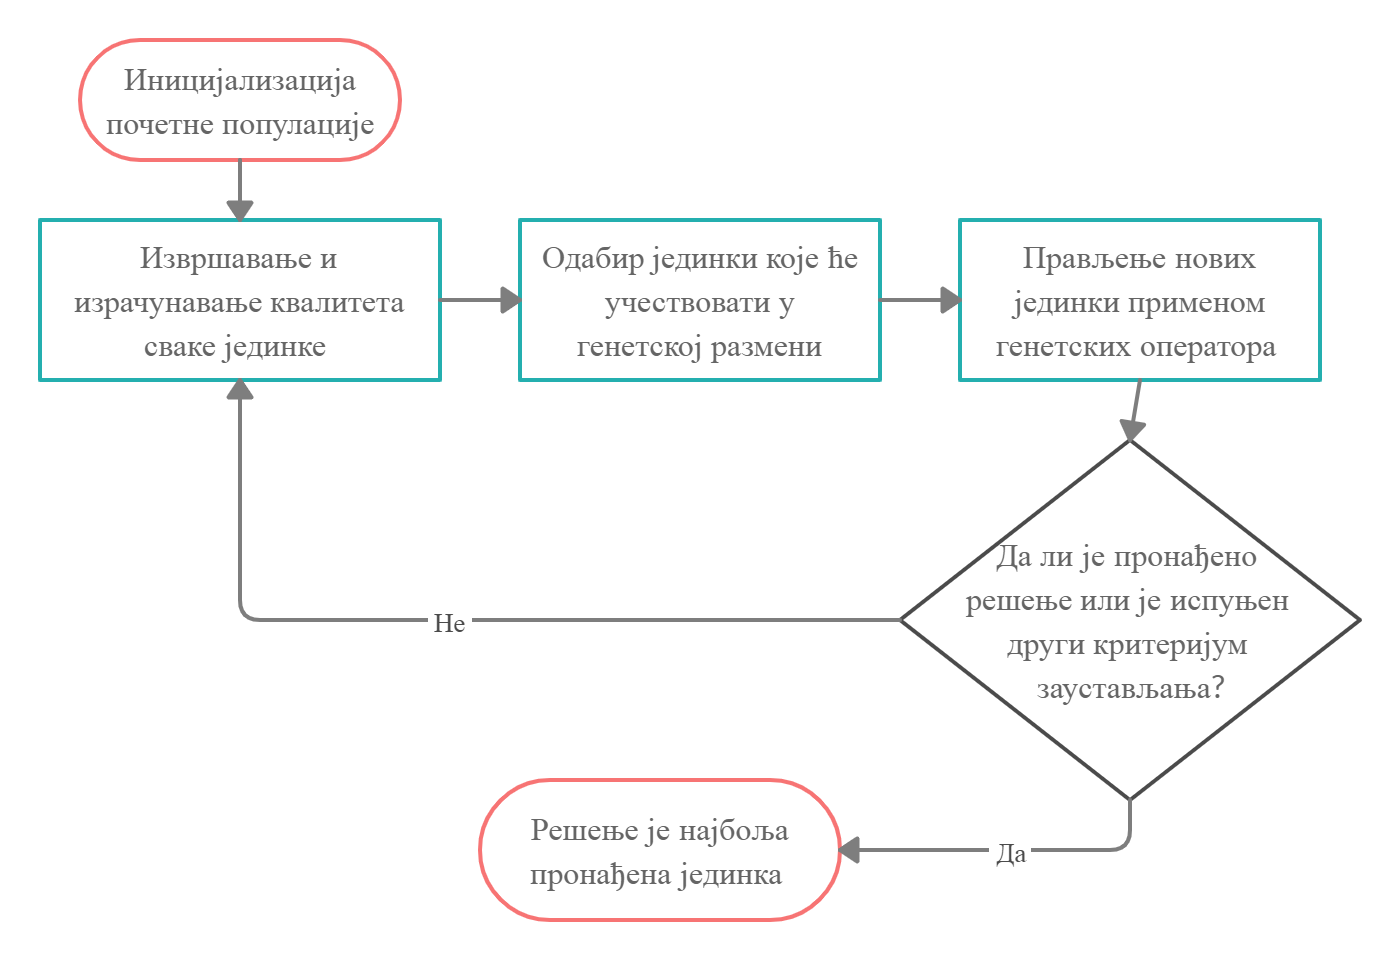
\includegraphics[scale=0.14]{opsti_algoritam.png}
        \end{center}
    \end{frame}
    
    \subsection[Репрезентација јединки]{Репрезентација јединки}

    \begin{frame}{Опис алгоритма}
    \end{frame}
    
    \subsection[Иницијализација популације]{Иницијализација популације}

    \begin{frame}{Опис алгоритма}
    \end{frame}

    \begin{frame}{Опис алгоритма}
    \end{frame}
    
    \begin{frame}{Опис алгоритма}
    \end{frame}

\section{Примери примене и мета-генетичко програмирање}

    \begin{frame}{Примери примене и мета-генетичко програмирање}
    \end{frame}

    \begin{frame}{Примери примене и мета-генетичко програмирање}
    \end{frame}

    \begin{frame}{Примери примене и мета-генетичко програмирање}
    \end{frame}
    
    \begin{frame}{Примери примене и мета-генетичко програмирање}
    \end{frame}
    
\section{Литература}
    \nocite{*}
    \begin{frame}{Литература}
        \printbibliography
    \end{frame}
    
\section{}
\begin{frame}{}
    \centering
        \Huge\bfseries{Хвала на пажњи!\\ Питања?}
\end{frame}
\end{document}





































\iffalse
\section{Some \LaTeX{} Examples}

\subsection{Tables and Figures}

\begin{frame}{Tables and Figures}

\begin{itemize}
\item Use \texttt{tabular} for basic tables --- see Table~\ref{tab:widgets}, for example.
\item You can upload a figure (JPEG, PNG or PDF) using the files menu. 
\item To include it in your document, use the \texttt{includegraphics} command (see the comment below in the source code).
\end{itemize}

% Commands to include a figure:
%\begin{figure}
%\includegraphics[width=\textwidth]{your-figure's-file-name}
%\caption{\label{fig:your-figure}Caption goes here.}
%\end{figure}

\begin{table}
\centering
\begin{tabular}{l|r}
Item & Quantity \\\hline
Widgets & 42 \\
Gadgets & 13
\end{tabular}
\caption{\label{tab:widgets}An example table.}
\end{table}

\end{frame}

\subsection{Mathematics}

\begin{frame}{Readable Mathematics}

Let $X_1, X_2, \ldots, X_n$ be a sequence of independent and identically distributed random variables with $\text{E}[X_i] = \mu$ and $\text{Var}[X_i] = \sigma^2 < \infty$, and let
\[ S_n = \frac{X_1 + X_2 + \cdots + X_n}{n}
      = \frac{1}{n}\sum_{i}^{n} X_i \]
denote their mean. Then as $n$ approaches infinity, the random variables $\sqrt{n}(S_n - \mu)$ converge in distribution to a normal $\mathcal{N}(0, \sigma^2)$.

\end{frame}
\fi
